\documentclass[border=0cm]{standalone}
\usepackage{tikz}
\tikzset{
    dot/.style={
        draw, scale=0.4, shape=circle, color=black, fill=black
    },
    center/.style={
        draw, scale=0.1, shape=circle, color=red, fill=red
    },
    blues/.style={
        color=blue
    },
    pair/.style={
        line width=1
    }
}
\definecolor{light-gray}{gray}{0.65}

% points...
\newcommand{\PA}{0.14/8.08, 0.25/6.49, 0.4/8.08, 0.73/6.19, 1.5/5.71, 1.58/4.84, 1.84/4.86, 2.12/7.69, 2.22/7.03, 2.31/5.74, 2.33/9.39, 2.45/7.36, 2.46/8.79, 2.72/6.36, 2.92/5.01, 2.99/7.21, 3.01/9.17, 3.13/7.25, 3.2/4.54, 3.26/7.98, 3.62/6.01, 3.62/7.95, 3.72/7.75, 4.04/7.42, 4.4/6.85, 4.57/8.6, 4.61/4.24, 4.8/7.03, 4.81/5.31, 4.81/7.73, 4.97/4.73, 5.17/6.33, 5.55/7.48, 5.58/4.63, 5.62/6.54, 5.74/9.45}
\newcommand{\PB}{4.04/7.42, 4.4/6.85, 4.57/8.6, 4.61/4.24, 4.8/7.03, 4.81/5.31, 4.81/7.73, 4.97/4.73, 5.17/6.33, 5.55/7.48, 5.58/4.63, 5.62/6.54, 5.74/9.45, 6.1/7.3, 6.29/6.26, 6.33/4.54, 6.34/7.23, 6.35/9.26, 6.47/8.94, 6.52/7.98, 6.73/8.33, 6.9/6.35, 6.95/4.16, 7.3/9.37, 7.35/7.97, 7.45/8.33, 7.59/9.08, 7.6/9.23, 7.72/7.19, 7.76/4.56, 7.77/7.29, 8.02/9.94, 8.52/5.94, 8.58/8.18, 8.75/8.26, 8.84/7.97, 8.94/5.37, 9.25/4.87, 9.45/8.86, 9.53/5.13, 9.72/7.49, 9.86/9.02}
\newcommand{\PC}{0.99/3.71, 1.28/2.31, 1.33/3.46, 1.43/2.06, 1.49/3.59, 1.5/5.71, 1.58/4.84, 1.75/3.73, 1.84/4.86, 1/2.52, 2.31/5.74, 2.33/3.59, 2.6/2.06, 2.88/1.81, 2.91/2.54, 2.92/5.01, 3.2/4.54, 3.28/2.57}
\newcommand{\PD}{1.5/5.71, 1.58/4.84, 1.75/3.73, 1.84/4.86, 2.31/5.74, 2.33/3.59, 2.6/2.06, 2.88/1.81, 2.91/2.54, 2.92/5.01, 3.2/4.54, 3.28/2.57, 3.69/3.83, 4.19/3.52, 4.22/2.43, 4.46/3.44, 4.61/4.24, 4.81/1.82, 4.81/5.31, 4.88/1.68, 4.97/4.73, 5.58/4.63, 5.82/3.61}
\newcommand{\PE}{1.28/2.31, 1.33/3.46, 1.43/2.06, 1/2.52, 2.05/0.41, 2.51/1.31, 2.6/2.06, 2.88/1.81, 2.91/2.54, 3.28/2.57}
\newcommand{\PF}{2.05/0.41, 2.51/1.31, 2.6/2.06, 2.88/1.81, 2.91/2.54, 3.28/2.57, 3.65/1, 4.22/2.43, 4.46/3.44, 4.77/0.02, 4.81/1.82, 4.84/0.26, 4.88/1.68}
\newcommand{\PG}{4.19/3.52, 4.22/2.43, 4.46/3.44, 4.61/4.24, 4.77/0.02, 4.81/1.82, 4.81/5.31, 4.84/0.26, 4.88/1.68, 4.97/4.73, 5.58/4.63, 5.82/3.61, 6.09/0.42, 6.16/3.21, 6.24/0.78, 6.33/4.54, 6.36/2.06, 6.95/4.16, 7.02/1.2, 7.08/3.47, 7.32/2.51, 7.34/3.12, 7.56/3.88, 7.76/4.56, 8.04/2.21, 8.23/2.09, 8.52/5.94, 8.94/5.37, 9.25/4.87, 9.53/5.13}
% grids...

% gap...
\newcommand{\eps}{1}
\newcommand{\gap}{1.1}
\newcommand{\dx}{0.1}
\newcommand{\dy}{0.1}

\begin{document}
    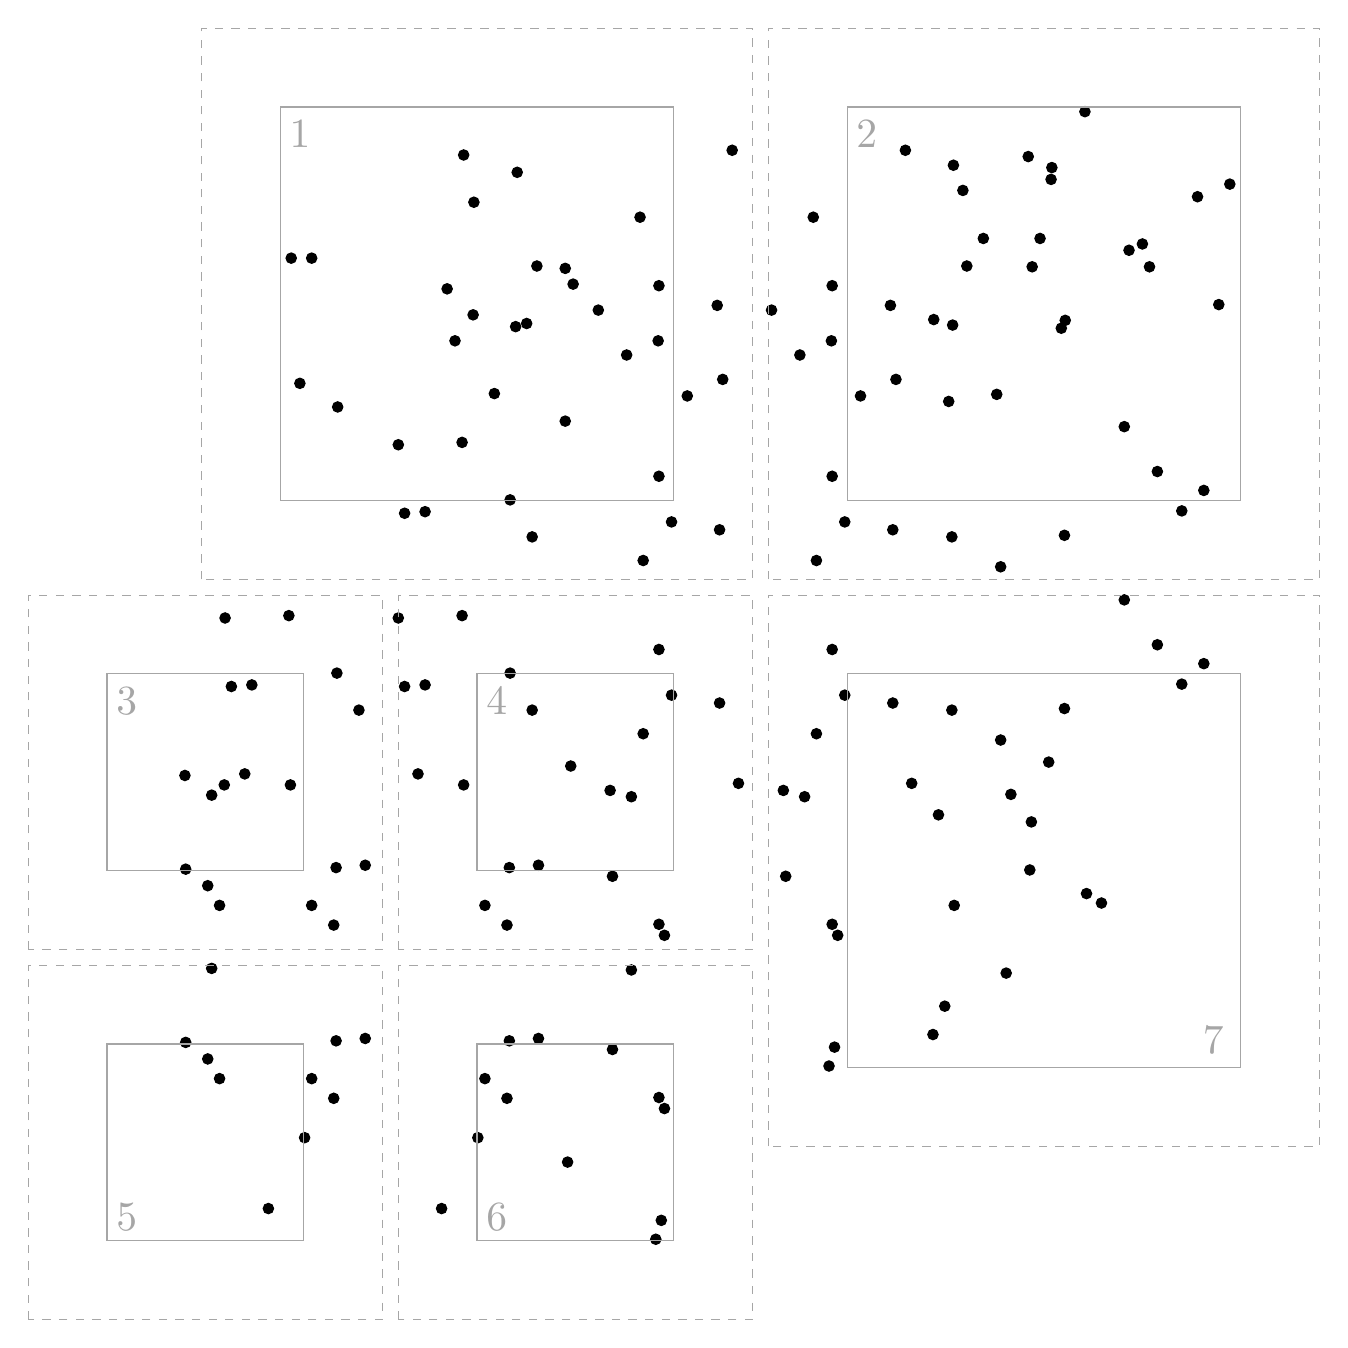
\begin{tikzpicture}
        \foreach \x/\y [count=\k from 0] in \PA { \coordinate[dot] (p\k) at (\x-\gap,\y+\gap); }
        \draw[light-gray] (0-\gap,5+\gap) rectangle (5-\gap,10+\gap);
        \draw[light-gray, dashed] (0-\gap-\eps,5+\gap-\eps) rectangle (5-\gap+\eps,10+\gap+\eps);
        
        \foreach \x/\y [count=\k from 0] in \PB { \coordinate[dot] (p\k) at (\x+\gap,\y+\gap); }
        \draw[light-gray] (5+\gap,5+\gap) rectangle (10+\gap,10+\gap);
        \draw[light-gray, dashed] (5+\gap-\eps,5+\gap-\eps) rectangle (10+\gap+\eps,10+\gap+\eps);
        
        \foreach \x/\y [count=\k from 0] in \PC { \coordinate[dot] (p\k) at (\x-\gap-\eps-\gap-\dx,\y-\gap); }
        \draw[light-gray] (0-\gap-\eps-\gap-\dx,2.5-\gap) rectangle (2.5-\gap-\eps-\gap-\dx,5-\gap);
        \draw[light-gray, dashed] (0-\gap-\eps-\gap-\eps-\dx,2.5-\gap-\eps) rectangle (2.5-\gap-\eps-\gap+\eps-\dx,5-\gap+\eps);
        
        \foreach \x/\y [count=\k from 0] in \PD { \coordinate[dot] (p\k) at (\x-\gap,\y-\gap); }
        \draw[light-gray] (2.5-\gap,2.5-\gap) rectangle (5-\gap,5-\gap);
        \draw[light-gray, dashed] (2.5-\gap-\eps,2.5-\gap-\eps) rectangle (5-\gap+\eps,5-\gap+\eps);

        \foreach \x/\y [count=\k from 0] in \PE { \coordinate[dot] (p\k) at (\x-\gap-\eps-\gap-\dx,\y-\gap-\eps-\gap-\dy); }
        \draw[light-gray] (0-\gap-\eps-\gap-\dx,0-\gap-\eps-\gap-\dy) rectangle (2.5-\gap-\eps-\gap-\dx,2.5-\gap-\eps-\gap-\dy);
        \draw[light-gray, dashed] (0-\gap-\eps-\gap-\eps-\dx,0-\gap-\eps-\gap-\eps-\dy) rectangle (2.5-\gap-\eps-\gap+\eps-\dx,2.5-\gap-\eps-\gap+\eps-\dy);
        
        \foreach \x/\y [count=\k from 0] in \PF { \coordinate[dot] (p\k) at (\x-\gap,\y-\gap-\eps-\gap-\dy); }
        \draw[light-gray] (2.5-\gap,0-\gap-\eps-\gap-\dy) rectangle (5-\gap,2.5-\gap-\eps-\gap-\dy);
        \draw[light-gray, dashed] (2.5-\gap-\eps,0-\gap-\eps-\gap-\eps-\dy) rectangle (5-\gap+\eps,2.5-\gap-\eps-\gap+\eps-\dy);

        \foreach \x/\y [count=\k from 0] in \PG { \coordinate[dot] (p\k) at (\x+\gap,\y-\gap); }
        \draw[light-gray] (5+\gap,0-\gap) rectangle (10+\gap,5-\gap);
        \draw[light-gray, dashed] (5+\gap-\eps,0-\gap-\eps) rectangle (10+\gap+\eps,5-\gap+\eps);
        
        \node[scale=1.5, color=light-gray] at (-0.85,10.75) {1};
        \node[scale=1.5, color=light-gray] at (6.35,10.75) {2};
        \node[scale=1.5, color=light-gray] at (-3.05,3.55) {3};
        \node[scale=1.5, color=light-gray] at ( 1.65,3.55) {4};
        \node[scale=1.5, color=light-gray] at (-3.05,-3) {5};
        \node[scale=1.5, color=light-gray] at ( 1.65,-3) {6};
        \node[scale=1.5, color=light-gray] at (10.75,-0.75) {7};
    \end{tikzpicture}
\end{document}
